\label{sec:intro}
\subsection{Context}
Drones, or Unmanned Aerial Vehicles (UAVs), are not new technologies. UAVs are currently used extensively, for both offensive\cite{ref:offence} and defensive\cite{ref:defence} operations, by militaries across the globe. There is also a strong push for UAVs in commercial applications, such as package delivery\cite{ref:package} and agriculture\cite{ref:agriculture}, and an ever-growing population of hobbyists\cite{ref:hobby}, adventurers\cite{ref:adventure} and athletes\cite{ref:sport} using UAV-mounted cameras to capture everything from weddings to skiing down mountains. However, there are several applications where current UAV technology just can't compete.\\

Rotor-based aircraft like the DJI Phantom (Figure \ref{fig:dji}) are notorious for their  large power demands and low range/flight time, making them difficult to use in applications requiring long distance travel, such as package delivery. Wing-based aircraft such as the HobbyKing Tornado\cite{ref:tornado} (Figure \ref{fig:tornado}) can achieve much greater travel distances as a result of higher efficiency flight. The biggest drawback of these aircraft, though, is they require open spaces (runways) to land safely, making them difficult to use in cramped or obstacle-rich applications such as low-altitude search in cities or bushland.

\begin{figure}[!ht]
	\centering
	\begin{minipage}{.5\textwidth}
		\centering
		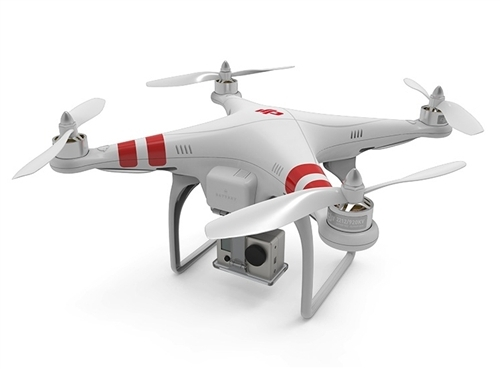
\includegraphics[width=134pt]{\IMAGEPATH /Aircraft/djiPhantom}
		\caption{DJI Phantom, a commercially available UAV}
		\label{fig:dji}
	\end{minipage}%
	\begin{minipage}{.5\textwidth}
		\centering
		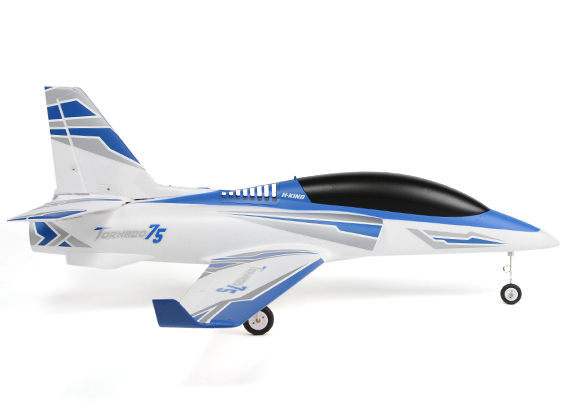
\includegraphics[width=206pt]{\IMAGEPATH /Aircraft/tornado}
		\caption{HobbyKing Tornado RC Plane}
		\label{fig:tornado}
	\end{minipage}
\end{figure}
 
The UAV Challenge\cite{ref:challenge}, organised by the Queensland University of Technology and the CSIRO, is a biennial competition that aims to push the boundaries of current autonomous aircraft technology. The 2016 challenge is titled ``Medical Express'', and charges teams with solving the issues raised above.\\

Competitors must develop an aircraft that can fly to a known area (up to 30km away) through specific transit corridors, search for and correctly identify ``Outback Joe'', land close to him in an obstacle-rich area to accept a pre-prepared blood sample, and then fly back to base. All of these actions must be completed within one hour, and must be autonomous; that is, after receiving the ``start'' signal the aircraft must have no human input. Table \ref{tab:challenge} highlights the key dates and corresponding stages of the UAV Challenge.\\

\begin{table}[!ht]
	\caption{UAV Challenge Timeline}
	\label{tab:challenge}
	\centering
	\begin{tabular}{ | l | l | }
		\hline
		\textbf{Events} & \textbf{Date} \\ \hline \hline
		Registration and Deliverable 1: Short Technical Report & \textit{Completed} \\ \hline
		Deliverable 2: Technical Report and Video & 13th April 2016 \\ \hline
		Deliverable 3: Autonomous Flight Record & 3rd August 2016 \\ \hline
		Final ``Go/No-Go'' decision for teams & 10th August 2016 \\ \hline
		Medical Express Challenge & Week starting 19th September 2016 \\
		\hline
	\end{tabular}
\end{table}

\subsection{Project Outline}
This project involves the development of an autonomous Unmanned Aerial Vehicle (UAV) with the capabilities to compete in the 2016 UAV Challenge. Given the Challenge specifications above, a number of design and performance requirements were identified that aircraft must meet in order to be successful:
\begin{enumerate}[label=\bfseries R\arabic*:] \itemsep-2pt
	\item Aircraft must be autonomous
	\item Take-off and landing in obstacle-rich environments (i.e. without a runway)
	\item Total flight endurance of at least 60km
	\item Total flight duration of up to 60 minutes
	\item Automated in-flight identification of a known target
	\item Ability to receive 500g payload upon landing
\end{enumerate}

It is anticipated that there will be several Capstone student teams continuing development of the UAV in 2016. Given the requirements listed above, and the timeline of the Challenge, this project sought to develop a working prototype with which to achieve the basic functionality required to compete in the Challenge. As such, the following objectives were selected for the project:
\begin{enumerate}[label=\bfseries O\arabic*:] \itemsep-2pt
	\item Register for the 2016 UAV Challenge
	\item Development of a prototype UAV for future teams to build on
	\item Development of autonomous flight controls to achieve \textbf{R1}
	\item Development of a novel hybrid flight system, incorporating both Vertical Take-Off and Landing (VTOL) and Fixed-Wing flight modes, for future teams to build upon to achieve requirements \textbf{R2}, \textbf{R3} and \textbf{R4}
	\item Development of in-flight search and obstacle avoidance mechanisms to be able to achieve \textbf{R5}
\end{enumerate}

The remaining sections of the report will discuss the work conducted by \ID in developing a working prototype for the UAV Challenge, beginning with a brief review of existing approaches that motivated the design of the UAV developed in this project. The following sections will discuss the various development domains of the UAV, including its design, flight and planning systems, and sensing systems, with a particular focus on the novel transition system developed for hybrid flight. The report will end with the results achieved by team \ID, work to be completed, and recommendations for 2016 teams in continuing the UAV's development.